\documentclass[10pt]{beamer}

\usetheme[sectionpage=none,
          subsectionpage=progressbar,
          progressbar=frametitle,
          numbering=fraction,
          block=fill]{metropolis}

\usepackage{polski}
\usepackage[polish]{babel}

\usepackage{pgfplots,
            smartdiagram}

\usesmartdiagramlibrary{additions}
\pgfplotsset{width=7cm,
            compat=1.8}


\usepackage{lipsum,
            hanging,
            amsmath,
            setspace,
            booktabs,
            xcolor}

\renewcommand{\arraystretch}{1.2}
\setstretch{1.1}

\makeatletter
  \setlength{\metropolis@titleseparator@linewidth}{2pt}
  \setlength{\metropolis@progressonsectionpage@linewidth}{2pt}
  \setlength{\metropolis@progressinheadfoot@linewidth}{2pt}
\makeatother

\definecolor{gray}{HTML}{716b58}
\definecolor{bar}{HTML}{c2b385}

\setbeamercolor{progress bar}{fg=bar}
\setbeamercolor{frametitle}{fg=white, bg=gray}

\setbeamertemplate{footnote}{%
  \hangpara{2em}{1}%
  \makebox[2em][l]{\insertfootnotemark}\footnotesize\insertfootnotetext\par%
}

\title[]
{
  Współczesne rozwiązania technologiczne pomagają w rozwoju i edukacji
}

\author[A.~Greloch \and W.~Zaremba \and M.~Zwierzyński \and J.~Lipski \and K.~Szturemski]
{
  A.~Greloch \and W.~Zaremba \and M.~Zwierzyński \and J.~Lipski \and K.~Szturemski
}

\institute[G1PIA]
{
  Klasa 3j\\
  Gimnazjum nr. 1 im. Powstańców Warszawy w Piasecznie
}

\date
{
  Piaseczno, 28 maja 2018
}

\begin{document}

\frame{\titlepage}

\begin{frame}{Spis treści}
\tableofcontents
\end{frame}

\section{Problem}
\subsection{Wprowadzenie do problematyki projektu}

\begin{frame}
  \frametitle{Problem}
  \begin{enumerate}
    \item Zbyt duża różnorodność treści w internecie $\rightarrow$ różna jakość i wiarygodność dostępnych informacji
    \item Zbyt duża popularność portali \textbf{typu social-learning}
    \item Za mała popularność rzetelnych internetowych źródeł wiedzy
    \item \textbf{Negatywna opinia o internecie jako medium naukowego}
  \end{enumerate}
  \begin{block}{Platformy social-learning'owe}
    Typ portalu społecznościowego, skupionego na udostępnianiu odpowiedzi do zadań z różnych przedmiotów tj. \emph{zadane.pl}, \emph{brainly.pl}, \emph{sciaga.pl}.
  \end{block}
\end{frame}

\begin{frame}
  \frametitle{Rzetelne internetowe źródła wiedzy}
  \small

  \begin{description}
    \item [\textbf{Platformy e-learning'owe}]\hfill\\ Typ portalu społecznościowego, skupionego na udostępnianiu materiałów edukacyjnych i opracowań z różnych dziedzin. Przykładem takiego portalu jest \emph{e-podreczniki.pl}.
    \item [\textbf{Encyklopedie, e-słowniki, e-biblioteki}]\hfill\\ Typ serwisu internetowego, udostępniającego zinformatyzowaną wersję źródeł naukowych oraz literackich. Przykładami takiego serwisu są \emph{wikipedia.org}, \emph{wolnelektury.net}, \emph{ebuw.uw.edu.pl} \footnote[frame]{e-biblioteka Uniwersytetu Warszawskiego}.
  \end{description}

\end{frame}

\begin{frame}
  \frametitle{Powstawanie negatywnej opinii o internecie w szkołach}
  \large
  \centering
  Platformy social-learningowe \\
  $\downarrow$ \\
  Wykorzystywanie ich w celu przepisania odpowiedzi do zadań, bez uprzedniego wykonania ich \\
  $\downarrow$ \\
  Nieprzyswojenie i nieprzetworzenie zadanego materiału \\
  $\downarrow$ \\
  Zaburzenie systemu nauczania \\
  $\downarrow$ \\
  Problem \\
  $\downarrow$ \\
  \textbf{Negatywna opinia nauczycieli o internecie jako ogóle}

\end{frame}

\begin{frame}
  \frametitle{Konsekwencje popularności serwisów social-learningowych}
  \begin{enumerate}
    \item Utrudnienie pracy nauczycielom
    \item Zmniejszenie wydajności systemu nauczania
    \item Niska jakość przyswajanego materiału
    \item Wypieranie rzetelnych źródeł wiedzy
  \end{enumerate}
  \begin{block}{Materiał}
    Tu: określone zagadnienie z podstawy programowej, które nauczyciel musi przerobić w ciągu roku szkolnego.
  \end{block}
\end{frame}

\section{Aplikacja}
\subsection{Przedstawienie aplikacji}

\begin{frame}
  \frametitle{ultraCALC: Aplikacja projektowa}
  Osiągnięte cele programistyczne:
  \begin{enumerate}
    \item Dynamiczne przeliczanie zmiennych \footnote[frame]{Algorytm, którego wynikiem jest wskazanie brakującej zmiennej oraz obliczenie jej.}
    \item Przetwarzanie definicji w czasie rzeczywistym \footnote[frame]{Przetworzenie surowych informacji, pochodzących z bazy danych, do interfejsu graficznego.}
    \item Dynamiczny i modularny interfejs
    \item Publikacja w sklepie Google Play \footnote[frame]{Domyślna platforma z aplikacjami na system Android -  \emph{play.google.com}.}
  \end{enumerate}
\end{frame}

\begin{frame}
  \frametitle{ultraCALC: Aplikacja projektowa}
  Aplikacja została stworzona, aby:
  \begin{enumerate}
    \item Móc zebrać rzetelne statystyki ze środowiska szkolnego dla poparcia tezy projektu
    \item Znaleźć alternatywę dla platform social-learningowych
    \item Mieć satysfakcję z napisania działającej aplikacji...
  \end{enumerate}
  \begin{block}{Teza}
    Współczesne rozwiązania technologiczne pomagają w rozwoju i edukacji
  \end{block}
\end{frame}

\begin{frame}
  \frametitle{Interfejs}
    \begin{figure}[p]
      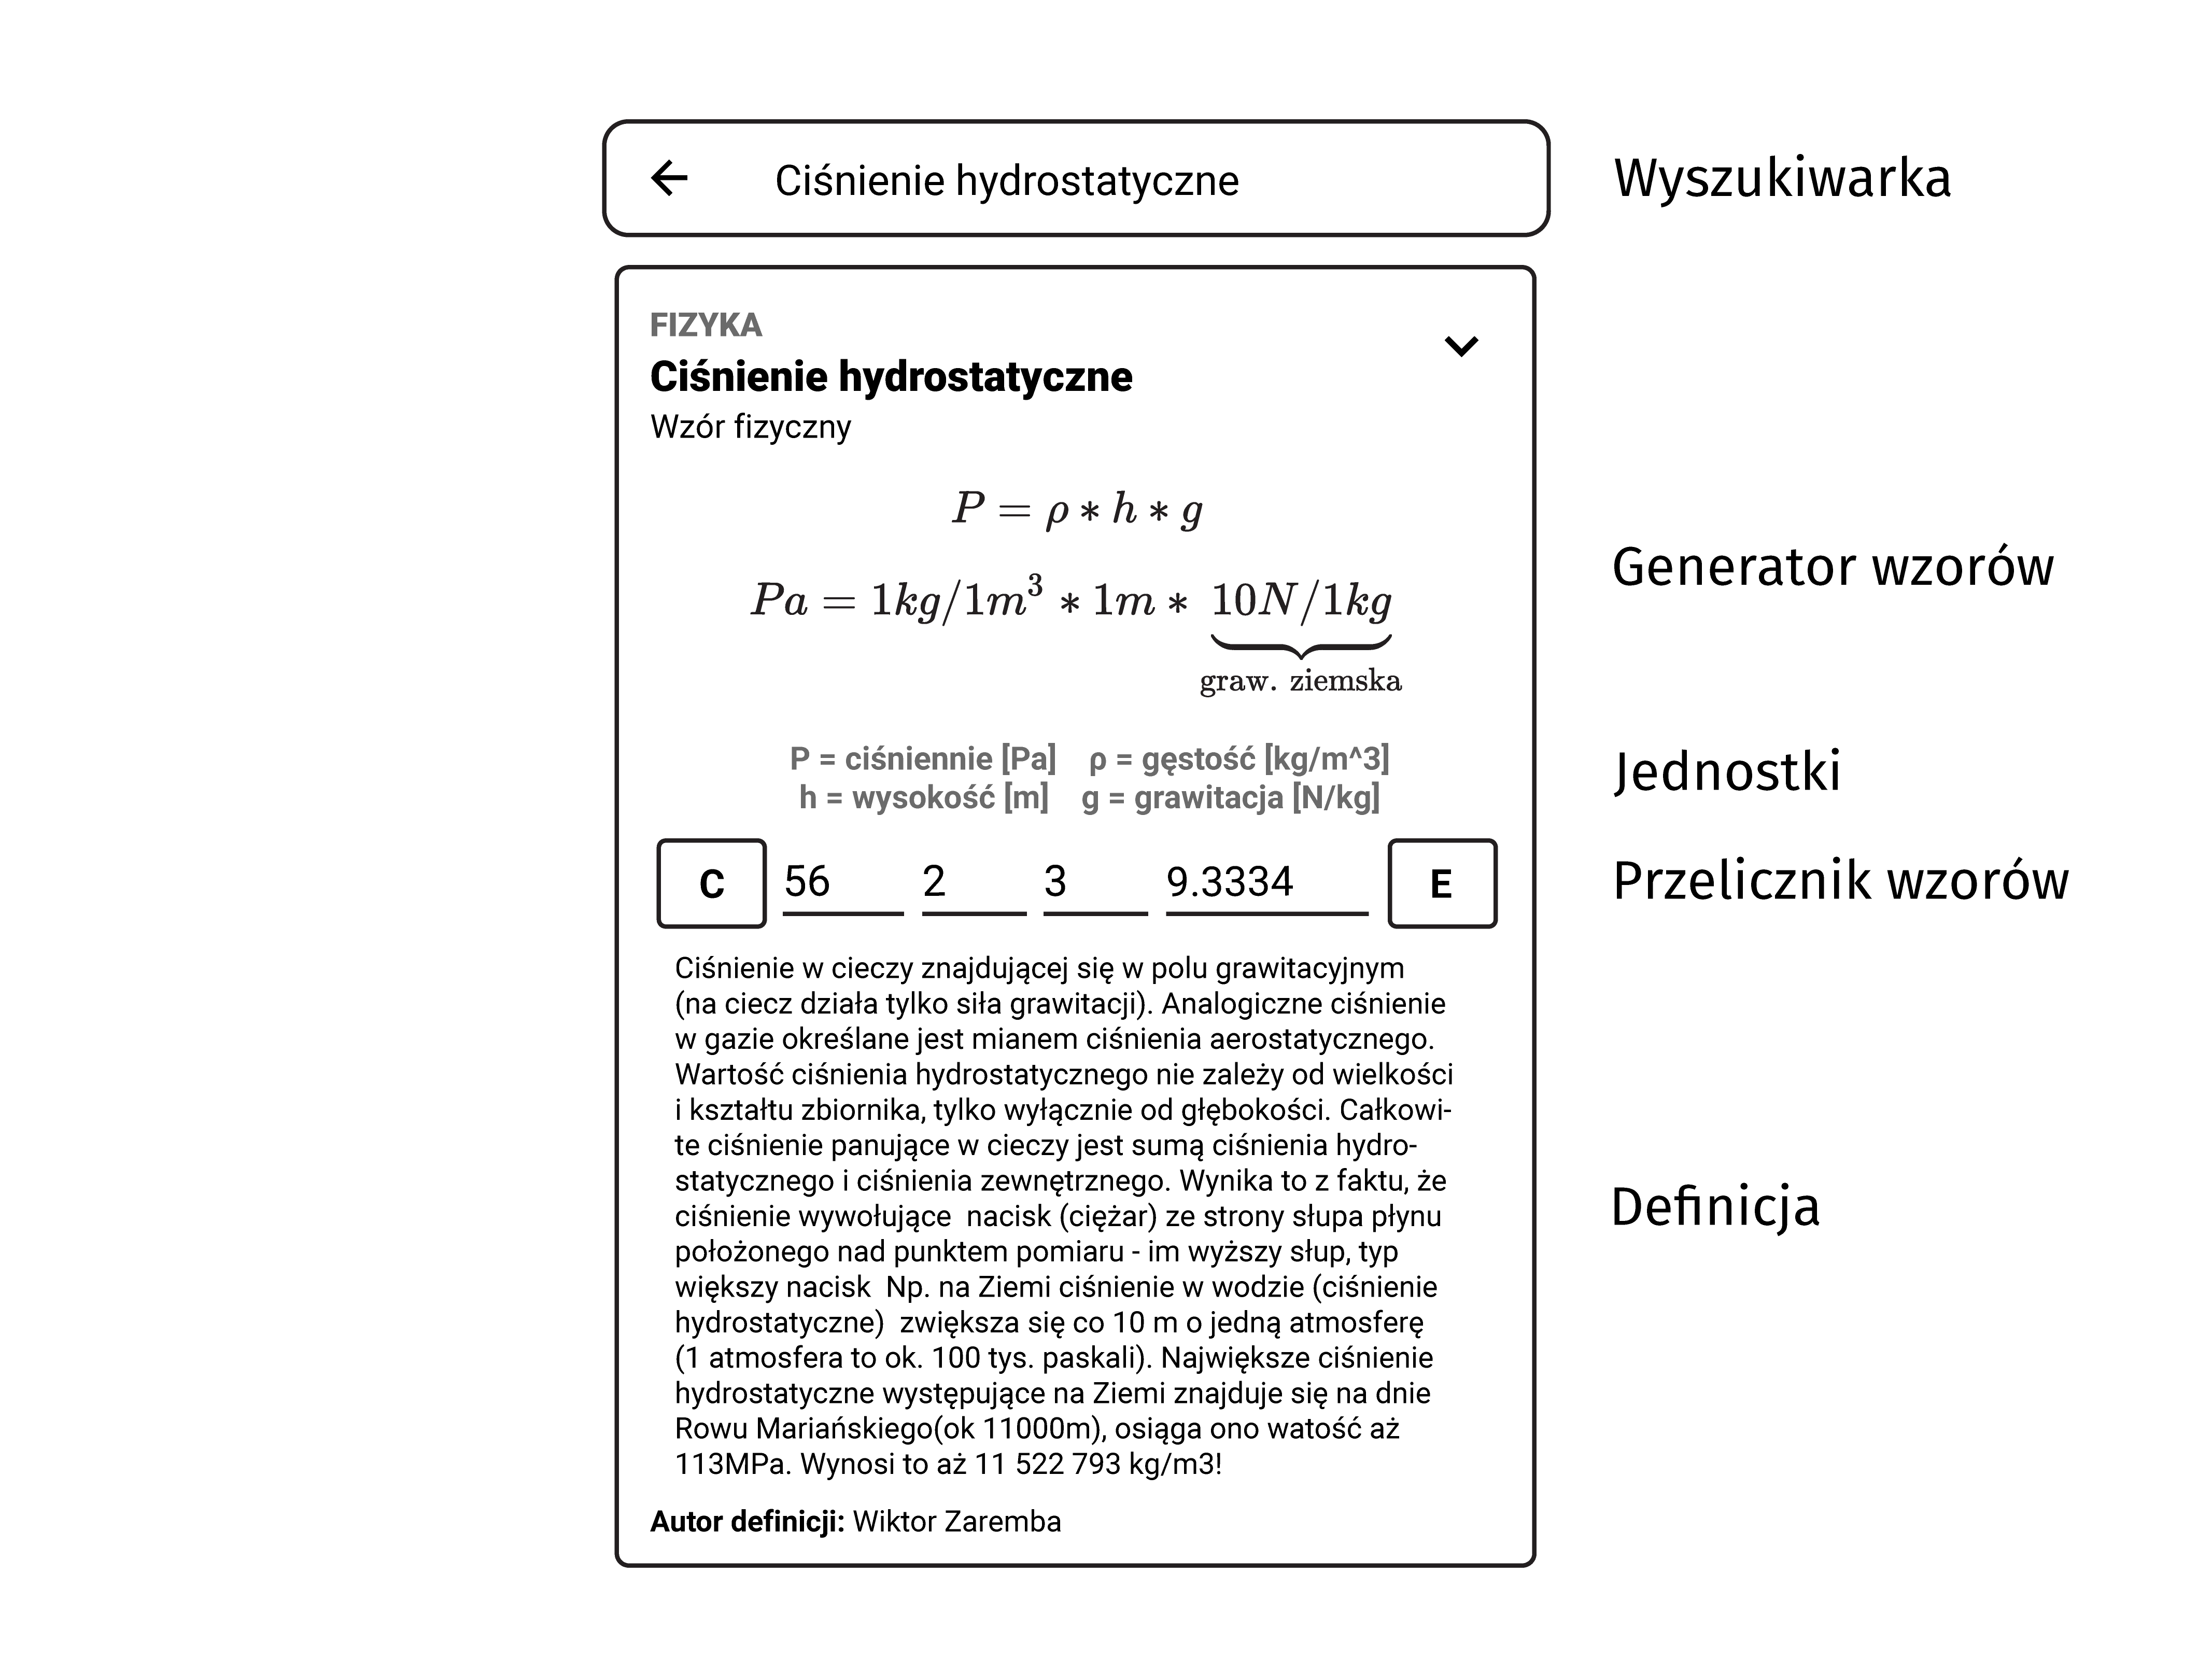
\includegraphics[width=10.5cm]{interfejs}
    \end{figure}
\end{frame}

\begin{frame}
	\tikzset{
	every shadow/.style={
		fill=none,
		shadow xshift=0pt,
		shadow yshift=0pt}
	}
  \smartdiagramset{
    circular distance=36mm,
    text width=80mm,
    font=\small,
    module minimum width=10mm,
    module minimum height=10mm,
    module shape=rectangle,
    uniform arrow color=true,
    arrow color=gray!50!black,
    border color=black,
    uniform color list=white for 6 items,
  }

  \frametitle{System nauki}
  	\begin{figure}[H]
  		\smartdiagram[flow diagram]{
		Pierwsza styczność z nowym zagadnieniem,
		Wykorzystywanie aplikacji przy wykonywaniu zadań,
 		Szybsze utrwalanie zagadnienia w praktyce,
 	   	Zrealizowanie materiału}
	\end{figure}

\end{frame}

\section{Doświadczenia}
\subsection{Przeprowadzenie testów z udziałem aplikacji w środowisku szkolnym}

\begin{frame}
\frametitle{Cele doświadczeń}
\begin{enumerate}
  \item Dowieść, że istnieją media internetowe, które wpływają korzystnie na proces przyswajania wiedzy
  \item Dowieść, że istnieją alternatywy dla platform social-learningowych
  \item Zaobserwować zachowania uczniów oraz ich oczekiwania wobec platform edukacyjnych
\end{enumerate}
\end{frame}

\begin{frame}
\frametitle{Sposób liczenia punktów}
\small
W doświadczeniu brały udział grupy dwu-, trzecio-, oraz czteroosobowe, dlatego brana pod uwagę jest ilość punktów przypadająca na jednego członka grupy.

$$\text{wynik} = \frac{\text{długość lekcji (45min)} - \text{czas (w minutach)}}{ (\frac{\text{ilość błędów}}{\text{maks. ilość pkt.}}+1) * \text{liczebność grupy}}$$

W dzieleniu dodawana jest wartość $+1$, aby uniknąć dzielenia przez $0$ w przypadku bezbłędnego rozwiązania wszystkich poleceń.

\textbf{Przykład:} Dwuosobowa grupa uczniów wykonała spośród czterech zadań matematycznych trzy dobrze. Niepoprawne wykonanie jednego zadania traktowane jest jako jeden błąd.

$$18.45 \approx \frac{45:00 - 3:30}{ (\frac{1}{4}+1) * \text{2}}$$
\end{frame}

\begin{frame}
  \begin{table}[H]
    \caption{Wyniki zadań fizycznych}
    \centering
    \begin{tabular}{@{}lllll@{}}
      \toprule
      Kategoria & Ilość punktów & Liczebność & Czas & Wynik \\
      \midrule
      internet & 2/2 & 2 & 13:58 & 18.5 \\
      aplikacja & 2/2 & 2 & 8:31 & 18.25 \\
      aplikacja & 2/2 & 2 & 10:08 & 17.44 \\
      aplikacja & 1/2 & 2 & 12.42 & 12.42 \\
      książka & 2/2 & 2 & 20:25 & 12.3 \\
      internet & 2/2 & 2 & 20:39 & 12.18 \\
      aplikacja & 1/2 & 2 & 17:38 & 10.95 \\
      książka & 0/2 & 2 & 12:40 & 10.78 \\
      książka & 1/2 & 3 & 20:50 & 9.67 \\
      \bottomrule
    \end{tabular}
  \end{table}

\end{frame}

\begin{frame}
  \begin{table}[H]
    \caption{Wyniki zadań matematycznych}
    \centering
    \begin{tabular}{@{}lllll@{}}
      \toprule
      Kategoria & Ilość punktów & Liczebność & Czas & Wynik \\
      \midrule
      aplikacja & 4/4 & 2 & 3:05 & 20.96 \\
      aplikacja & 4/4 & 2 & 4:10 & 20.42 \\
      internet & 3/4 & 2 & 3:30 & 18.45\\
      książka & 2/4 & 2 & 9:44 & 14.11 \\
      książka & 2/4 & 4 & 10:16 & 13.9 \\
      \bottomrule
    \end{tabular}
  \end{table}

\end{frame}

\begin{frame}
\frametitle{Średnia arytmetyczna wszystkich kategorii}

\begin{figure}[H]

\begin{tikzpicture}
	\begin{axis}
	[
	xbar,
	y axis line style = { opacity = 0 },
	axis x line       = none,
	tickwidth         = 0pt,
	enlarge y limits  = 0.7,
	enlarge x limits  = 0.2,
	nodes near coords,
	symbolic y coords = {Fizyka,Matematyka},
	legend style={at={(1,0.0)},
	legend cell align={left},
	anchor=south west},
	ytick=data
	]
	\addplot coordinates { (20.69,Matematyka) (14.77,Fizyka) };
	\addplot coordinates { (18.45,Matematyka) (15.34,Fizyka) };
	\addplot coordinates { (14.01,Matematyka) (10.92,Fizyka) };
	\legend{Aplikacja, Internet, Książka}
  \end{axis}
\end{tikzpicture}

\end{figure}

\tiny Na podstawie danych zebranych z klasy 7A oraz 7D. Zespołów wykorzystujących aplikacji z obu klas było łącznie $6$, wykorzystujących tylko internet $4$ a korzystających z samej książki oraz kalkulatora $7$.

\end{frame}

\section{Podsumowanie}
\subsection{Końcowe wnioski oraz omówienie wyników doświadczeń}

\begin{frame}
  \frametitle{Wnioski i końcowe obserwacje}
  \begin{enumerate}
    \item Z zadaniami matematycznymi uczniowie klas siódmych poradzili sobie znacznie lepiej niż z zagadnieniami fizycznymi
    \item Aplikacja uzyskała zainteresowanie zgodne z naszymi oczekiwaniami ($\sim 100$ instalacji w tym 47 aktywnych użytkowników do dnia dzisiejszego)
    \item Uczniowie są otwarci na nowe sposoby nauczania i są chętni je testować
  \end{enumerate}
\end{frame}

\begin{frame}
  \frametitle{Wpływ na social-learning}
  Doświadczenia wykazały, że uczniowie nie są stale przywiązani do platform social-learningowych.

  Oznacza to, że jest możliwe wyparcie tego typu serwisów i przywrócenie dawnej wydajności nauczania przy użyciu alternatywnych rozwiązań.

  \raggedleft Dziękujemy za uwagę.
\end{frame}

\end{document}
